\documentclass{article}

\usepackage[%
    left=0.5in,%
    right=0.5in,%
    top=0.5in,%
    bottom=0.5in,%
]{geometry}%
\usepackage{minitoc}
\usepackage{multicol}
\usepackage{graphicx}
\usepackage{fixltx2e}
\usepackage{listings}
\usepackage{color}
\usepackage{hyperref}
    \hypersetup{ colorlinks = true, linkcolor = blue }
\usepackage{blindtext}
\definecolor{lightgray}{gray}{0.9}
\graphicspath{ {./} }

\newcommand{\inlinecode}[2]{\colorbox{lightgray}{\lstinline
[language=#1]$#2$}}
\newcommand{\worddef}[1]{\hyperref[sec:reference]{\textit{#1}}}

\begin{document}

\tableofcontents

\newpage

\section{How can we save power for mobiles}

\begin{itemize}
  \item Knowledge about the power consumption of each component and app 
  \item Screen /network/CPU off or release other device resources as soon as not needed 
  \item Limit resources for less frequently used apps 
  \item Set device to sleep as soon as no user interactions 
  \item Global management of running jobs across all apps (i.e. perform syncs, upload/download together at fixed time window)
\end{itemize}

\subsection{Battery Consumption Statistics}

\begin{itemize}
  \item Framework tracks the time that devices spend in different states (e.g. WiFi chipset:on/off, Display :low/high brightness) 
  \item Controlling service pushes state changes to BatteryStats service. Framework pulls the data at these transition points 
  \item App consumption power is calculated based on CPU run time at specific speeds
\end{itemize}

\section{Android Power Management Concept}

\begin{itemize}
  \item  Designed for mobile devices 
  \item Goal is to prolong battery life 
  \item Based on Linux Power Management (\textbf{not suitable for a mobile device})
  \begin{itemize}
    \item – G0 (working) 
    \item – G1 (sleeping)
    \begin{itemize}
      \item S1 (CPU stops executing instructions, power to CPU and RAM maintained) 
      \item S2 (CPU powered off, cache is flushed) 
      \item S3 (Standby / sleep / suspend to powered RAM) 
      \item S4 (Hibernate / suspend to disk, RAM powered off) –
    \end{itemize}
    \item - G2 (S5, soft off) 
    \item – G3 (mechanical off) 
   \end{itemize}  
  \item Mobile phones have a default “off” behaviour
\end{itemize}

\subsection{Power Management Design}

\begin{multicols}{2}

\begin{itemize}
  \item A wrapper to Linux Power Management 
  \item Added to the Kernel – Wake Lock mechanism 
  \item Apps need to request CPU \& Screen to be on with WakeLocks, otherwise Android will shut down the CPU 
  \item Wake locks and timeouts constantly switch the state of the system’s power
  \begin{itemize}
    \item Overall system power consumption decreases
    \item “Better” use of battery capacity
  \end{itemize}
\end{itemize}

\vfill\null

\begin{center}
  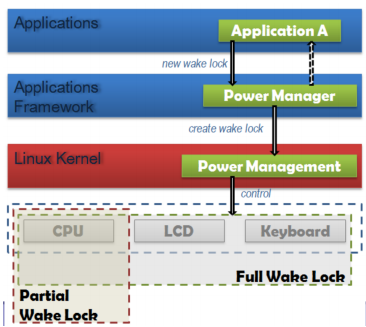
\includegraphics[scale=0.5]{power_architecture.png}
\end{center}

\end{multicols}

\section{Battery Life Enhancement in Android (Android 6.0 onwards)}

\begin{itemize}
  \item \textbf{App Standby}: defer background activity for apps with no recent user interaction. 
  \item \textbf{Doze}: deep sleep if user has not actively used the device for extended periods of time 
  \item \textbf{Exemptions}: system apps and cloud messaging services preloaded on phone are exempted from App Standby \& Doze. 
  \item Test apps in App standby \& Doze mode for the desired performance
\end{itemize}

\section{App Standby}

\begin{itemize}
  \item \textbf{Start conditions}: an app is not actively used for a certain time will be placed in an idle mode
  \begin{itemize}
    \item Not doing foreground work (activities/service, pending notifications)
    \item Hasn’t been explicitly launched for certain time (days). 
  \end{itemize}
  \item \textbf{Actions}: No network access, no background jobs, can set Alarms, can use wake locks, allow network access once per day 
  \item \textbf{Exists conditions}: plug in the device, do some foreground tasks
\end{itemize}

\subsection{App Standby Buckets (Android 9.0)}

\begin{flushleft}
Prioritize apps based on how recently and how frequently the apps are used
\begin{itemize}
  \item Active: currently or recently used 
  \item Working Set: regular use 
  \item Frequent: often used not everyday 
  \item Rare: not frequently 
  \item Never: never
\end{itemize}

\section{Doze}

\begin{itemize}
  \item \textbf{Starts Doze}: when device is in idle - screen off, on battery \& stationary. 
  \item \textbf{In Doze}: no network access; no CPU-intensive work; wakelocks ignored; no wifi scan; deferred alarm manager alarms; only high priority notification received; no job scheduler; no sync adapters. 
  \item \textbf{Exits Doze}: user interaction, device motion, screen on, or AlarmClock alarm. Notification do not cause Doze exits. 
  \item \textbf{Maintenance window}: complete pending activities (syncs, jobs, etc). • MMS/SMS/Telephony services are excluded from Doze
\end{itemize}

\section{Exemptions}

\begin{itemize}
  \item System apps and cloud messaging services preloaded on phone are exempted from App Standby \& Doze. 
  \item Use whitelist for apps to be partially exempt from Doze \& App Standby
  \begin{itemize}
    \item \verb|isIgnoringBatteryOptimiztions()| to check if in the whitelist;
    \item \verb|ACTION_IGNORE_BATTERY_OPTIMIZATION_SETTINGS| intent to direct user to battery optimization options 
    \item \verb|REQUEST_IGNORE_BATTERY_OPTIMIZATIONS| allow user to add app to whitelist directly 
  \end{itemize}
  \item Whitelisted apps can use network and hold partial wake locks during Doze \& App Standby, but jobs \& syncs are still deferred. 
  \item App should not be on the whitelist unless can’t use FCM high-priority messages or App’s core function is affected
\end{itemize}

\end{flushleft}

\section{Sustained Performance Mode (new API in Android 7.0)}
\begin{itemize}
  \item \textit{Thermal throttling prevents} a long running apps maintain its performance (e.g. game, camera, virtual reality application etc.) 
  \item App can request the platform to enter a SPM, and keep a consistent level of performance
  \begin{itemize}
    \item Only tests on Android 7.0 on Nexus 6P devices 
    \item Set using \verb|Window.setSustainedPerformanceMode()|
    \item System automatically disables the mode when no longer in focus
  \end{itemize}
\end{itemize}

\pagebreak
\section*{Reference section} \label{sec:reference}
\begin{description}
	\item[placeholder] \hfill \\
\end{description}
\end{document}
